The patient is Patient-007, the first in id order with all five phases and a three-image DSCR item (a rule fixed before any answer was inspected). Figure~\ref{fig:v4example} shows the images the models see and the donor images used in the swap; each item is four-way multiple choice, with the full stems and options in the reproducibility artifact.

\paragraph{AIA (positive control).} Which MRI sequence does this image show? \emph{Key:} D) T1-weighted, after gadolinium contrast.

\paragraph{LIL.} Where is the main tumor region (enhancing tumor, necrosis or resection cavity, not the surrounding edema) on this slice? \emph{Key:} A) Right hemisphere, posterior half.

\paragraph{DSCR.} What is the response category at follow-up? \emph{Key:} B) Progressive disease.

The key comes from the bidimensional products of the tracked lesion on the three slices (10, 0 and 385\,mm$^2$ at baseline, nadir and follow-up); there is no measurable enhancing disease at the nadir and a measurable lesion at follow-up (a new measurable lesion), which the rule calls progressive disease. The expert rating is PD (``Target L.: 1, 16mm x 19mm''), the same category, so this is not an audit disagreement.

\paragraph{TCM.} Using your earlier assessment of this patient, what is the most appropriate next step? \emph{Key:} C) Change therapy now: bring re-resection, second-line treatment or a clinical trial to tumor board.

The stem states the patient facts (see the artifact) and the rule: non-PD $\rightarrow$ continue; PD and $\le$ 12 weeks after radiotherapy $\rightarrow$ repeat MRI first; PD and later $\rightarrow$ change therapy (RANO 2010; Stupp schedule assumed). Here the category is progressive disease and chemoradiotherapy ended 53 weeks before the scan, so the class is escalate; changing the stated timing across the 12-week window or the stated category changes the rule's answer (the fact flips of E3).

\paragraph{PJRF (secondary).} Same patient facts as TCM; the model forecasts the probability of death within 52 weeks of the scan (recorded outcome: death), scored by the Brier score.

\paragraph{Donor swap.} Each image is replaced by a donor's whose key differs (AIA Patient-054, FLAIR not T1c; LIL Patient-023, L post not R post; DSCR Patient-019, PR not PD); the stem and options are unchanged, so the donor's answer is always an option.


\begin{table}[t]
\centering
\scriptsize
\setlength{\tabcolsep}{3pt}
\begin{tabular}{lccc}
\toprule
 & AIA & LIL & DSCR \\
\midrule
Key/donor & T1c/FLAIR & R post/L post & PD/PR \\
\midrule
Gemini-3.6-Flash & T1c/T1c/FLAIR & R post/R ant/L post & PD/PD/CR \\
Llama-4-Scout & T1c/T1c/T1 & L post/L post/L post & PD/SD/PD \\
Gemma-3-27B & T2/T1c/FLAIR & L ant/L ant/L post & PD/PD/PD \\
Gemma-3-12B & T2/T2/FLAIR & R ant/R ant/L post & PD/PD/PD \\
MedGemma-4B & T1/T1/T1 & R ant/R ant/L ant & CR/CR/CR \\
\bottomrule
\end{tabular}
\caption{Answers for Patient-007 (own/text/swap in each cell), with the key and donor key; Gemini-3.6-Flash is the reference model. Labels: T1c is T1 after contrast; L/R hemisphere, ant/post half; PD, SD, PR, CR are RANO categories.}
\label{tab:v4example}
\end{table}



\begin{figure*}[t]
\centering
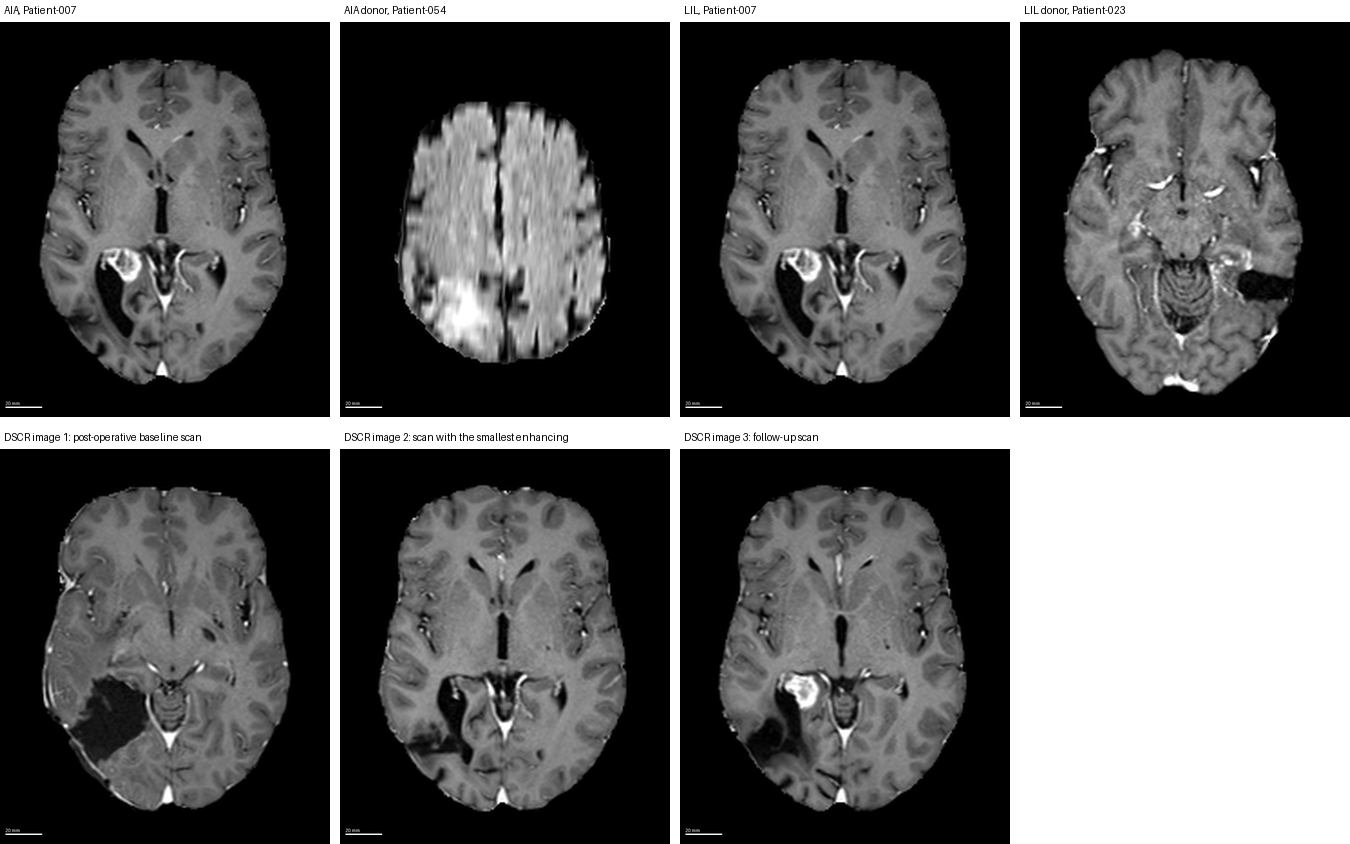
\includegraphics[width=\textwidth]{figures/v4_example}
\caption{Images for Patient-007. Top: the AIA slice and its donor, the LIL slice and its donor. Bottom: the three DSCR slices (baseline, nadir, follow-up). Slices are atlas-space, skull-stripped, magnified 4$\times$, with a 20\,mm scale bar.}
\label{fig:v4example}
\end{figure*}
